\subsubsection{Radars Operations}
\label{sec:osg_radars_ops} 

How to define radar attributes is defined in \nameref{sec:ui_configure_data_sources}. \\

For each defined radar, the following information can be shown:

\begin{itemize}
 \item Label text at center position
 \item Range rings (if defined)
\begin{itemize}
 \item Minimum/maximum range
 \item Colored for PSR in brown, SSR in blue, Mode S in purple
\end{itemize} 
\end{itemize} 
\ \\

The radars layer display configuration is stored in the configuration and restored upon startup. \\

To access the map operations, click the (top) radars symbol \includegraphics[width=0.5cm,frame]{../../data/icons/radar_black.png}, then the following operations are available:

\begin{itemize}
 \item Show All: Shows all radars
 \item Hide All: Hides all radars
 \item Toggle Labels: Shows/hides labels for all radars
 \item Toggle Range Rings: Shows/hides all range rings for all radars
\end{itemize} 

\begin{figure}[H]
    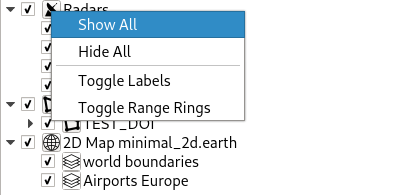
\includegraphics[width=8cm,frame]{figures/osgview_radars_ops.png}
  \caption{OSG View radars layer operations}
\end{figure}
